\documentclass[a4paper,12pt]{article}
\usepackage{lscape}
\usepackage[utf8]{inputenc}
\usepackage[T2A]{fontenc}
\usepackage[english,russian]{babel}
\usepackage[left=20mm, right=20mm, top=20mm, bottom=20mm]{geometry}
\usepackage{setspace}
\usepackage{comment}
\usepackage{amsmath}
\usepackage{tikz}
\usetikzlibrary {arrows.meta}
\usepackage{dashrule}
\usepackage{fancyhdr}%оформление отчёта
\usepackage{hyperref}%оформление отчёта
\usepackage{listings}
\usepackage{amssymb}
\usepackage{parskip}
\usepackage[T1]{fontenc}
\usepackage{textcomp,enumitem}
\usepackage{hyperref}
\usepackage{indentfirst}
\usepackage{graphicx}
\setlength{\parindent}{5ex}
\usepackage{algorithm}
\usepackage{algpseudocode}

\begin{document}
	\begin{center}
		\normalsize{Министерство образования и науки} \par
		\normalsize
		{Санкт-Петербургский политехнический университет Петра Великого} \par
		{Институт Компьютерных наук и кибербезопасности}\par
		{Высшая школа технологий искусственного интеллекта}\par
		{Направление 02.03.01 Математика и Компьютерные науки}
	\end{center}
	\vfill
    
	\begin{center}
		{\large Отчёт по дисциплине \guillemotleft Алгоритмические основы компьютерной графики\guillemotright}\par
		{\huge   Лабораторная работа №4
		
		\guillemotleft Моделирование в среде UNITY\guillemotright}\par
        
	\end{center}
	\vfill
	\begin{flushleft}
		Выполнил студент: \hspace{3.6cm} \rule[0pt]{2.5cm}{0.5pt} \hspace{0.0cm} Салимли Айзек Мухтар Оглы\par
		\vspace{0.2cm}
		Проверил: \hspace{5.4cm} \rule[0pt]{2.5cm}{0.5pt} \hspace{0.1cm} Курочкин Михаил Александрович
	\end{flushleft}
	\vspace{0.5cm}
	\begin{flushright}
		\guillemotleft \rule[0pt]{0.8cm}{0.5pt}\guillemotright \rule[0pt]{2cm}{0.5pt} 20\rule[0pt]{0.5cm}{0.5pt} г.
	\end{flushright}
	\vfill
	\begin{center}
		Санкт-Петербург, 2025
	\end{center}
	\thispagestyle{empty}
	\newpage
	\tableofcontents
	\newpage
	
	\section*{Введение}\addcontentsline{toc}{section}{Введение}
	
	Графический движок — это программное обеспечение, специально разработанное для управления и рендеринга графики в компьютерных приложениях, включая видеоигры, симуляторы, анимации, виртуальную реальность и многие другие. Графические движки предоставляют набор инструментов и функций, которые упрощают и ускоряют процесс создания визуальных элементов и эффектов в приложении.
	
	Целью данной работы является изучение графического движка UNITY. Изначально стояла цель изучения UNIGINE, но так как моя операционная система не позволяет его установить, то движок был замене на аналогичный — UNITY.
	
	\textbf{Постановка задачи:}
	\begin{itemize}
		\item Ознакомиться с 3D-движком UNITY и возможностями, которые он предоставляет;
		 \item Импортировать в UNITY модели, разработанные в ходе выполнения лабораторной работы №1;
		  \item Создать сцену с импортированными объектами
	\end{itemize}
	
	\newpage
\section{Описание сценария}

В сцене присутствуют четыре основных твёрдых объекта — колпачок, фигурка динозавра, карандаш и поверхность.

У каждого объекта заданы физические свойства: включена гравитация, заданы масса, форма и материал с упругостью.

\begin{itemize}
    \item \textbf{Колпачок}: масса $m_1 = 100\,$г, физическая форма — коническая. Присвоен физический материал с коэффициентом упругости $e = 0{,}8$.
    \item \textbf{Фигурка динозавра}: масса $m_2 = 280\,$г, форма — объемная с широкой нижней площадью. Коэффициент упругости $e = 0{,}6$.
    \item \textbf{Карандаш}: масса $m_3 = 200\,$г, форма — цилиндрическая. Коэффициент упругости $e = 0{,}7$.
    \item \textbf{Поверхность}: идеально плоская, неподвижная, с коэффициентом упругости $e = 0{,}5$.
\end{itemize}

В начальный момент времени колпачок, фигурка динозавра и карандаш висят на небольшой высоте над поверхностью друг над другом.

С началом сцены объекты начинают свободное падение под действием силы тяжести. Первой приземляется фигурка динозавра — она падает плашмя и остаётся на месте. Карандаш падает сверху на фигурку и начинает скатываться из-за своей цилиндрической формы. Затем сверху на него падает колпачок, частично отскакивает, раскручивается и откатывается в сторону, после чего останавливается.

Все объекты в сцене обладают упругостью. При столкновениях между ними используются правила упругого удара. Для определения скорости отскока применяется следующая формула:

\[
v_{\text{после}} = e \cdot v_{\text{до}}
\]

где:
\begin{itemize}
    \item $v_{\text{до}}$ — скорость объекта до столкновения,
    \item $v_{\text{после}}$ — нормальная составляющая скорости после столкновения,
    \item $e$ — коэффициент упругости взаимодействующих тел (используется среднее значение двух объектов: $e = \frac{e_1 + e_2}{2}$).
\end{itemize}

Таким образом, все взаимодействия в сцене моделируются как частично упругие, обеспечивая реалистичное отскакивание и последующее гашение движения. Отскок колпачка и скатывание карандаша подчёркивают влияние формы и упругости на поведение тел.

В рассматриваемой сцене все столкновения между объектами являются \textbf{частично упругими}, так как коэффициент упругости $e$ всех материалов меньше 1.

При частично упругом столкновении происходит потеря части кинетической энергии: часть энергии переходит в теплоту, деформации и вращательное движение.

Общая кинетическая энергия системы после столкновений становится меньше, чем до них:

\[
E_{\text{кинетическая, после}} < E_{\text{кинетическая, до}}
\]

При этом выполняется закон сохранения импульса, но не сохраняется полная механическая энергия.

Таким образом, \textbf{кинетическая энергия частично теряется при взаимодействии объектов}, особенно в момент контакта колпачка с карандашом и последующего его отскока, а также при столкновении карандаша с фигуркой динозавра. Итоговое поведение тел демонстрирует постепенное затухание движения и переход в состояние покоя.

Сцена не предполагает разрушений — все объекты остаются целыми. Демонстрируется только влияние гравитации и взаимодействий тел с учётом упругих столкновений.

	
	\newpage
	\section{Описание UNITY}
	
	Unity — это популярный многоплатформенный 3D-движок, широко используемый для создания игр, интерактивных приложений, систем виртуальной и дополненной реальности, а также интерактивной визуализации и симуляторов в различных областях.
	
	Unity совместим с различными операционными системами, включая Microsoft Windows, macOS и Linux, что делает его доступным для разработчиков на самых разных платформах. Движок поддерживает множество графических API, таких как DirectX, OpenGL, Vulkan и Metal, что обеспечивает гибкость и высокое качество графики на различных устройствах.
	
	Одним из ключевых преимуществ Unity является его мощный и интуитивно понятный интерфейс, а также обширный набор инструментов для разработки. Unity включает в себя визуальный редактор, который позволяет разработчикам создавать и редактировать сцены и игровые миры в режиме реального времени. Это существенно ускоряет процесс разработки и упрощает работу с проектами.
	
	Unity поддерживает несколько языков программирования, что делает его доступным для широкой аудитории разработчиков. С помощью C\# можно создавать сложные игровые механики и интерактивные элементы, что позволяет реализовать практически любые идеи.
	
	Движок предоставляет мощные инструменты для работы с визуальными эффектами, такими как шейдеры, освещение и постобработка, что способствует созданию реалистичной и привлекательной графики. Unity также включает в себя модуль физики, который позволяет моделировать столкновения, динамику твердых тел, жидкости и ткани, а также управлять другими физическими взаимодействиями в игре.
	
	Unity обладает обширной экосистемой, включающей в себя Unity Asset Store, где разработчики могут приобретать и продавать различные ресурсы, такие как модели, текстуры, звуки и скрипты. Это позволяет значительно ускорить процесс разработки, используя готовые решения и наработки.
	
	Кроме того, Unity поддерживает разработку для множества платформ, включая ПК, консоли, мобильные устройства, веб-браузеры и устройства виртуальной и дополненной реальности. Это дает разработчикам возможность создавать игры и приложения, которые могут быть выпущены на самых различных устройствах, охватывая широкую аудиторию пользователей.
	
	Таким образом, Unity представляет собой мощный и гибкий инструмент для разработки, предлагая широкий спектр возможностей для создания высококачественных и интерактивных 3D-приложений на самых разных платформах.
	
	\newpage
	\section{Устройство проекта UNITY}
	
		 Unity - это интегрированная среда разработки, предоставляющая всё необходимое для создания впечатляющих мультимедийных проектов, начиная от игр и заканчивая симуляциями и визуализациями. Проект в Unity представляет собой центральную единицу, объединяющую код, ассеты (контент) и настройки приложения.
	
	\begin{itemize}
		
	

	
	\item Unity использует систему координат для определения положения объектов в виртуальном пространстве. Трехмерное пространство описывается системой координат с осями X, Y и Z, где X и Y образуют горизонтальную плоскость, а Z указывает направление вверх. Это позволяет разработчикам точно позиционировать объекты в сцене и управлять их движением и взаимодействием.
	
	\item Сцены в Unity - это виртуальные пространства, где происходит визуализация и взаимодействие объектов. Сцены в Unity содержат различные элементы, такие как модели, источники света, камеры и другие объекты. Они организованы в иерархическое дерево, что позволяет создавать сложные визуальные композиции и управлять отношениями между объектами.
	
\item В Unity каждый объект представляет собой сущность, существующую в виртуальном мире, и может иметь различные компоненты, определяющие его внешний вид, поведение и взаимодействие с другими объектами. Объекты могут содержать геометрические меши, текстуры, скрипты, коллайдеры и другие компоненты, что позволяет создавать разнообразные и интерактивные сцены.
	
\item 	Геометрические меши в Unity представляют собой сетку полигонов, определяющих форму объекта.

Текстуры позволяют добавлять детали и цвета. Это позволяет разработчикам создавать реалистичные модели и окружения для своих проектов.
	
\item 	В Unity существует понятие поверхностей и материалов. Поверхность в Unity - это часть геометрии объекта, которая может иметь свой собственный материал или свойства. Каждая поверхность может быть настроена отдельно, что позволяет регулировать её внешний вид и свойства независимо от других поверхностей. Поверхности могут быть организованы в иерархию внутри общей сетки объекта, что позволяет, например, управлять уровнем детализации объекта.
	
\item 	Материал в Unity определяет внешний вид поверхности объекта и базируется на нескольких ключевых компонентах. Эти компоненты включают в себя шейдеры, текстуры, состояния и параметры. Шейдеры - это программы, которые определяют внешний вид материала при рендеринге. Текстуры используются для нанесения изображений на поверхности объектов, а параметры позволяют настраивать поведение и визуальные эффекты материала.
	
\item 	Также в Unity существует система физической симуляции, которая позволяет создавать реалистичные сценарии виртуального мира. Физическая модель в Unity основана на упрощенной ньютоновской физике и позволяет имитировать различные физические явления, такие как коллизии, столкновения, гравитацию и другие. Объекты в Unity могут иметь тела и формы, которые определяют их физические свойства и взаимодействие с окружающей средой. Это позволяет создавать интерактивные и реалистичные сцены, где объекты могут взаимодействовать между собой и с пользователем.
\end{itemize}

\newpage
\section{Реализация сцены}

\subsection{Создание проекта}
Для начала работы программы необходимо установить Unity Hub. Далее в Unity Hub нужно выбрать интерусующую нас версию Unity, я установил UNITY 2021.3.38f1.

После установки всех компонентов можно создать проект. UNITY проект — это «контейнер» для кода, содержимого и мета-данных приложения.

Открываем проект и видим начальный мир (Рис.1).

\begin{center}
	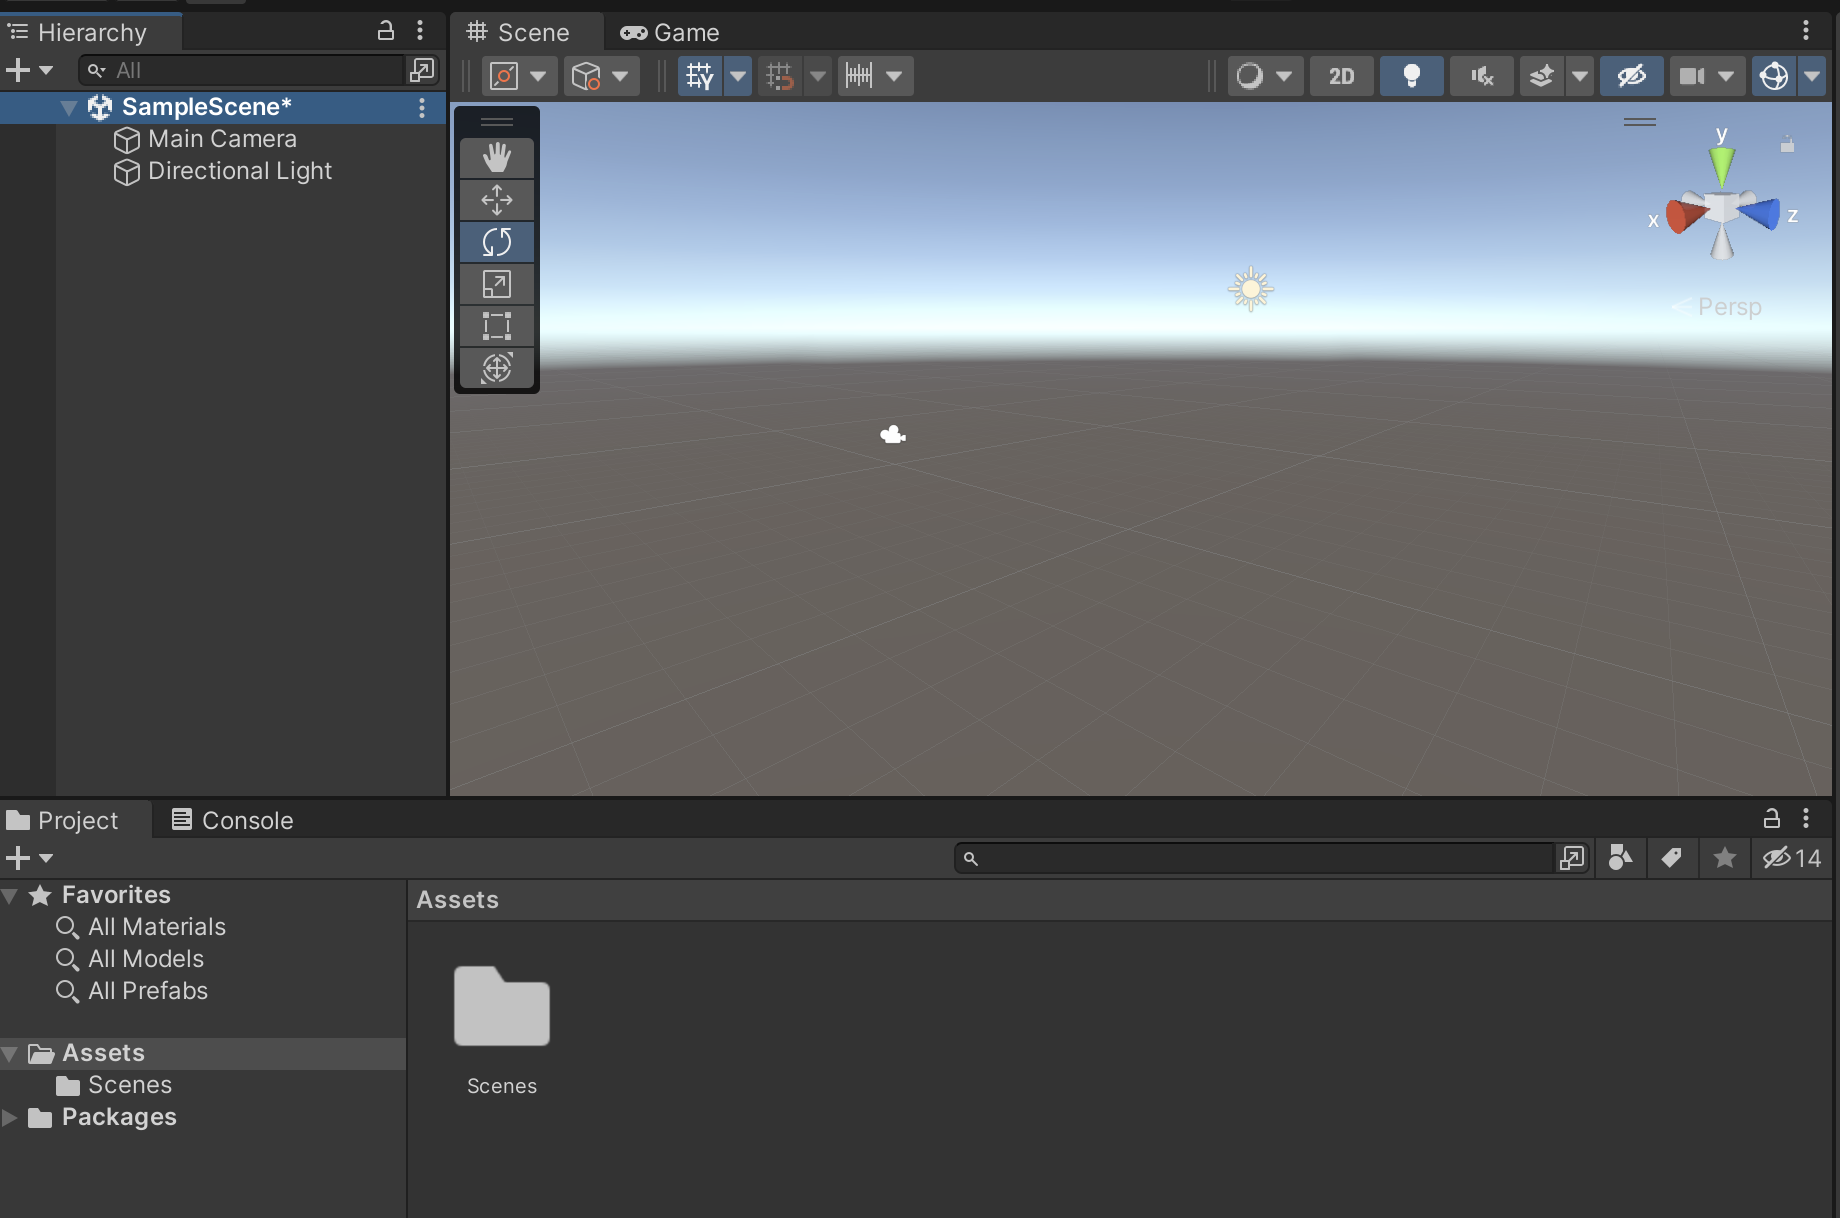
\includegraphics[scale = 0.5]{1.png}\\
	Рис.1 Начальный мир
\end{center}

\subsection{Экспорт моделей}

В ходе выполнения первой практической работы в Blender были разработы модели кактуса, лампы и ночника.

С этими предметами и реализуем сцену в Unity. Для этого импортируем предметы, загрузив их в папку Assets, далее они появяится в рабочем окне и достаточно будет просто перетянуть их в мир. Импортированные модели на рис.2.


\begin{center}
	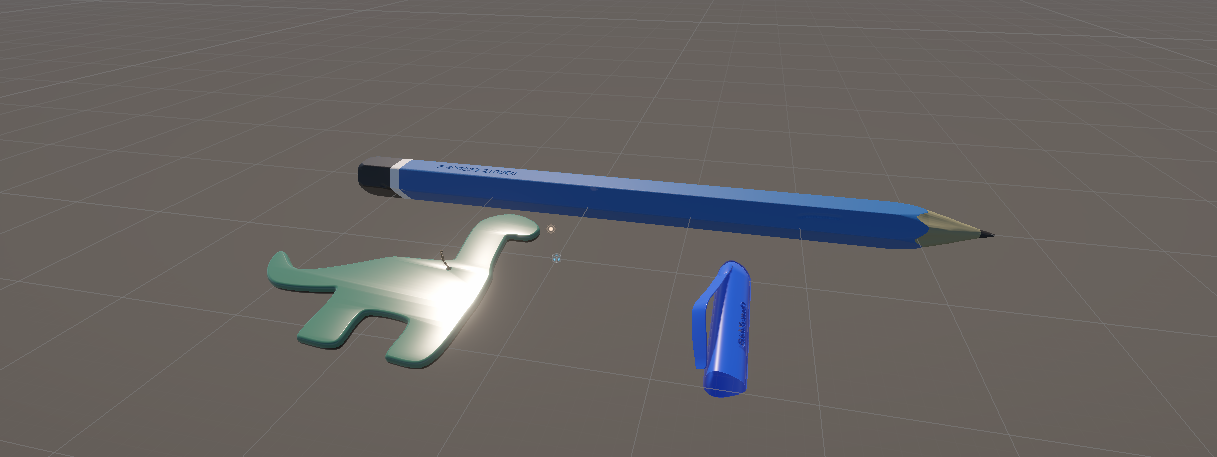
\includegraphics[scale = 0.4]{2.png}\\
	Рис.2 Импортированные модели
\end{center}

Теперь создадим твердую поверхность, на которой модели будут стоять или падать на нее впсоледствии. Для этого на левой боковой панели нажмем + —> 3D Object —> Plane. 

\begin{center}
	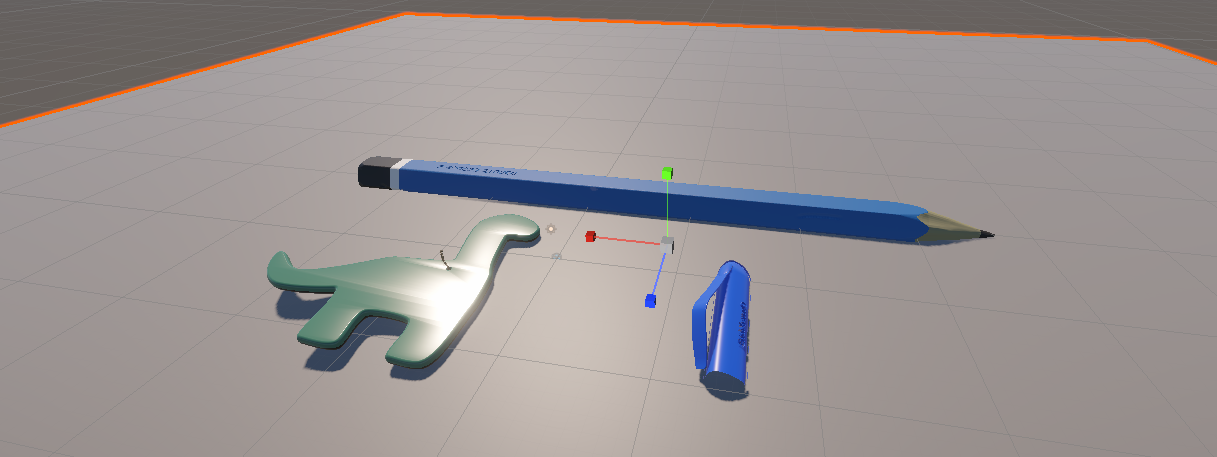
\includegraphics[scale = 0.4]{3.png}\\
	Рис.3 Создание поверхности
\end{center}

\subsection{Физика моделей}

Теперь самое основное, необхлдимо задать физику объектов, чтобы они могли взаимодействовать друг с другом и с поверхностью. Так как сейчас это объекты без твердой оболочки, без гравитации, без массы.

Каждому из трех объектов необходимо задать два компонента:

\begin{enumerate}
	\item Rigidbody — отвечает за физику предмета, его массу и гравитацию.
	\item Collider — задает форму объекта.
\end{enumerate}

\subsubsection{Физика фигурки динозавра}

Добавим Rigidbody Add Component —> Rigidbody и поставим галочку около Use Gravity, чтобы наш предмет мог падать/отскакивать и также быть подвластен гравитации, как и в реальной жизни. Также зададим массу.

Теперь зададим форму. Добавим  Add Component —> Box Collider, так как предмет больше всего вписывается в данную форму. 

Настройки фигурки представлены на Рис.4.

\begin{center}
	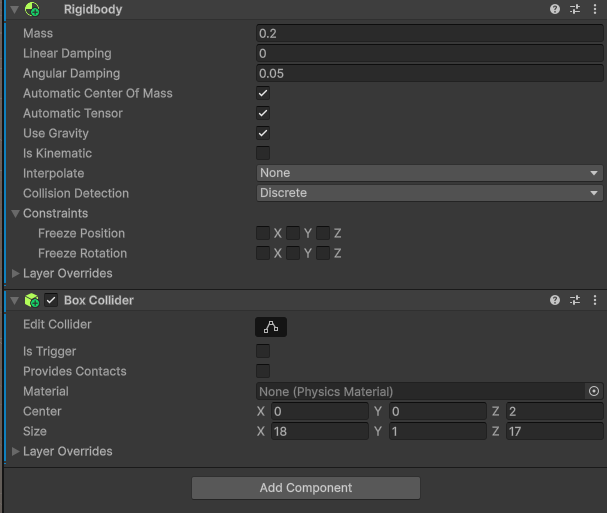
\includegraphics[scale = 0.5]{4.png}\\
	Рис.4 Физика фигурки динозавра
\end{center}


\subsubsection{Физика карандаша}

Добавим Rigidbody Add Component —> Rigidbody и поставим галочку около Use Gravity, чтобы наш предмет мог падать/отскакивать и также быть подвластен гравитации, как и в реальной жизни. Также зададим массу.

Теперь зададим форму. Добавим  Add Component —> Capsule Collider, так как предмет больше всего похож на данную форму.

Настройки карандаша представлены на Рис.5.

\begin{center}
	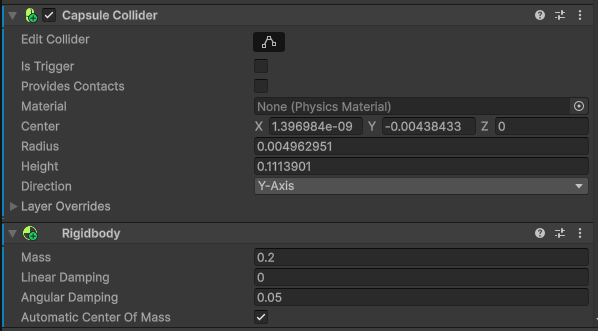
\includegraphics[scale = 0.5]{5.png}\\
	Рис.5 Физика карандаша
\end{center}

\subsubsection{Физика колпачка}

Добавим Rigidbody Add Component —> Rigidbody и поставим галочку около Use Gravity, чтобы наш предмет мог падать/отскакивать и также быть подвластен гравитации, как и в реальной жизни. Также зададим массу.

Теперь зададим форму. Добавим  Add Component —> Box Collider, так как предмет больше всего вписывается в данную форму. 

Настройки колпачка представлены на Рис.6.

\begin{center}
	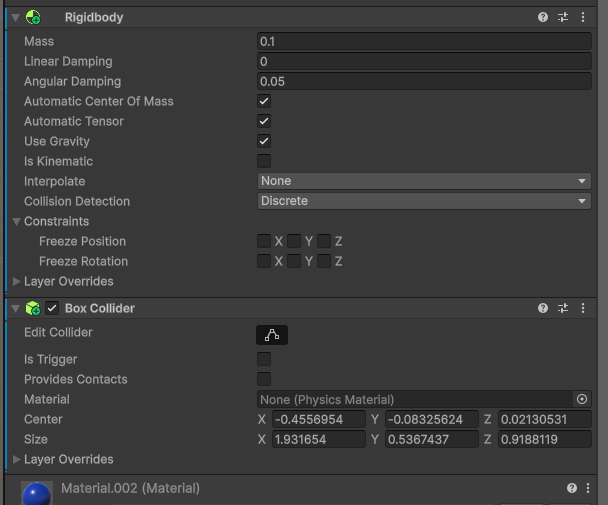
\includegraphics[scale = 0.5]{6.png}\\
	Рис.6 Физика колпачка
\end{center}

\subsection{Положение моделей}

Теперь необходимо расставить объекты в пространстве так, как было задумано в нашей сцене. Для этого нужно нажать на каждый объект и в Transform задать нужные параметры .

\begin{center}
	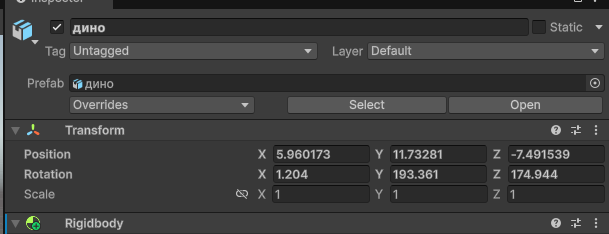
\includegraphics[scale = 0.5]{7.png}\\
	Рис.7 Положение фигурки динозавра
\end{center}

\begin{center}
	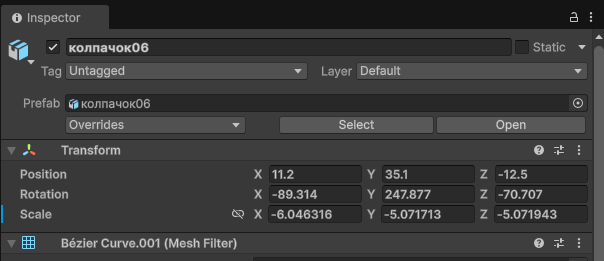
\includegraphics[scale = 0.5]{8.png}\\
	Рис.8 Положение колпачка
\end{center}

\begin{center}
	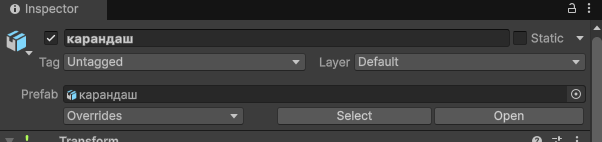
\includegraphics[scale = 0.5]{9.png}\\
	Рис.9 Положение канадаша
\end{center}

\newpage
\section{Результаты работы программы}

Запустим нашу сцену. В результате работы был получен .mp4 файл, содержащий полученную сцену. 

Результат работы программы предоставлен во внешнем файле "Видео лаб 4.mp4"

\newpage
	\section*{Заключение}\addcontentsline{toc}{section}{Заключение}
В ходе работы были освоены основы работы с 3D-движком UNUITY и его возможностями.

При создании сцены были импортированы три модели, которые ранее были созданы в Blender 3D: колпачок, фигурка динозвра и карандаш. Этим моделям были заданы физические свойства, такие как: форма, масса, инерция и тд.

Данная лабораторная работа позволила ознакомиться с инструментарием UNITY, а анализ поведения объектов в пространстве позволил лучше понять физическую модель объекта и использовать это для создания сцены.

\newpage
	\section*{Список источников}\addcontentsline{toc}{section}{Список источников}
	
[1] Unity Documentation: https://docs.unity.com (дата обращения: 25.05.2025)
\end{document}